\documentclass[11pt]{report}
\usepackage[utf8]{inputenc}
\usepackage{graphicx}
\usepackage{amsmath}
\usepackage{booktabs}
\usepackage{float}
\usepackage[a4paper, top=2.5cm, bottom=2.5cm, left=2.5cm, right=2.5cm]{geometry}

\title{
    \vspace{2cm}
    \textbf{Machine Learning 441: Assignment 1} \\
    \large Data Exploration
}
\author{
    Ruan Buhr \\ 
    \small 26440873
}
\date{\today}

\begin{document}

\maketitle

\section*{Task 1: Data Quality Reports}

The \texttt{badDataSet.csv} data set contains 581012 instances, with 62 descriptive features and a single response.

\begin{table}[H]
\centering
\caption{Data Quality Report for the Descriptive Features.}
\label{tab:data_quality_report_des_feat}
\resizebox{\textwidth}{!}{
    \begin{tabular}{lrrrrrrrrrr}
\toprule
Feature & Count & \% Miss. & Card. & Min. & 1st Qrt. & Mean & Median & 3rd Qrt. & Max. & Std. Dev. \\
\midrule
A1 & 581012 & 0.00 & 1978 & 2054845.65 & 3104928.15 & 3271134.43 & 3311628.60 & 3496222.05 & 4264440.30 & 309481.13 \\
A2 & 578069 & 0.51 & 361 & 0.00 & 58.00 & 155.66 & 127.00 & 260.00 & 360.00 & 111.91 \\
A3 & 581012 & 0.00 & 576099 & 0.00 & 145.49 & 389.92 & 318.12 & 652.53 & 903.48 & 280.34 \\
A4 & 580708 & 0.05 & 67 & 0.00 & 9.00 & 14.10 & 13.00 & 18.00 & 66.00 & 7.49 \\
A5 & 578069 & 0.51 & 569 & -691.00 & 108.00 & 269.42 & 218.00 & 384.00 & 1397.00 & 212.56 \\
A6 & 581012 & 0.00 & 581012 & -173.07 & 6.99 & 46.42 & 29.91 & 68.97 & 600.95 & 58.30 \\
A7 & 578069 & 0.51 & 577988 & -1.00 & -0.50 & -0.00 & -0.00 & 0.50 & 1.00 & 0.58 \\
A8 & 581012 & 0.00 & 5811 & 0.00 & 1106.00 & 8158.11 & 1997.00 & 3328.00 & 510165098.00 & 1185156.02 \\
A9 & 578069 & 0.51 & 207 & 0.00 & 198.00 & 212.14 & 218.00 & 231.00 & 254.00 & 26.77 \\
A10 & 578069 & 0.51 & 186 & 0.00 & 213.00 & 223.32 & 226.00 & 237.00 & 254.00 & 19.77 \\
A11 & 581012 & 0.00 & 255 & 0.00 & 119.00 & 142.53 & 143.00 & 168.00 & 254.00 & 38.27 \\
A12 & 578069 & 0.51 & 5826 & 0.00 & 1024.00 & 1980.43 & 1710.00 & 2550.00 & 7173.00 & 1324.25 \\
A13 & 578069 & 0.51 & 2 & 0.00 & 0.00 & 0.45 & 0.00 & 1.00 & 1.00 & 0.50 \\
A14 & 581012 & 0.00 & 2 & 0.00 & 0.00 & 0.05 & 0.00 & 0.00 & 1.00 & 0.22 \\
A15 & 581012 & 0.00 & 2 & 0.00 & 0.00 & 0.44 & 0.00 & 1.00 & 1.00 & 0.50 \\
A16 & 578069 & 0.51 & 1 & 0.00 & 0.00 & 0.00 & 0.00 & 0.00 & 0.00 & 0.00 \\
A17 & 581012 & 0.00 & 1 & 0.00 & 0.00 & 0.00 & 0.00 & 0.00 & 0.00 & 0.00 \\
A18 & 578069 & 0.51 & 3 & 0.00 & 0.00 & 0.07 & 0.00 & 0.00 & 2.00 & 0.28 \\
A19 & 581012 & 0.00 & 2 & 0.00 & 0.00 & 0.50 & 0.00 & 1.00 & 1.00 & 0.50 \\
A20 & 577566 & 0.59 & 2 & 0.00 & 0.00 & 0.01 & 0.00 & 0.00 & 1.00 & 0.07 \\
A21 & 173355 & 70.16 & 2 & 0.00 & 0.00 & 0.01 & 0.00 & 0.00 & 1.00 & 0.07 \\
A22 & 581012 & 0.00 & 2 & 0.00 & 0.00 & 0.01 & 0.00 & 0.00 & 1.00 & 0.11 \\
A23 & 581012 & 0.00 & 2 & 0.00 & 0.00 & 0.01 & 0.00 & 0.00 & 1.00 & 0.09 \\
A24 & 581012 & 0.00 & 2 & 0.00 & 0.00 & 0.02 & 0.00 & 0.00 & 1.00 & 0.14 \\
A25 & 581012 & 0.00 & 2 & 0.00 & 0.00 & 0.00 & 0.00 & 0.00 & 1.00 & 0.05 \\
A26 & 581012 & 0.00 & 2 & 0.00 & 0.00 & 0.01 & 0.00 & 0.00 & 1.00 & 0.11 \\
A27 & 581012 & 0.00 & 2 & 0.00 & 0.00 & 0.00 & 0.00 & 0.00 & 1.00 & 0.01 \\
A28 & 581012 & 0.00 & 2 & 0.00 & 0.00 & 0.00 & 0.00 & 0.00 & 1.00 & 0.02 \\
A29 & 581012 & 0.00 & 2 & 0.00 & 0.00 & 0.00 & 0.00 & 0.00 & 1.00 & 0.04 \\
A30 & 581012 & 0.00 & 2 & 0.00 & 0.00 & 0.06 & 0.00 & 0.00 & 1.00 & 0.23 \\
A31 & 581012 & 0.00 & 2 & 0.00 & 0.00 & 0.02 & 0.00 & 0.00 & 1.00 & 0.14 \\
A32 & 581012 & 0.00 & 2 & 0.00 & 0.00 & 0.05 & 0.00 & 0.00 & 1.00 & 0.22 \\
A33 & 581012 & 0.00 & 2 & 0.00 & 0.00 & 0.03 & 0.00 & 0.00 & 1.00 & 0.17 \\
A34 & 581012 & 0.00 & 2 & 0.00 & 0.00 & 0.00 & 0.00 & 0.00 & 1.00 & 0.03 \\
A35 & 581012 & 0.00 & 2 & 0.00 & 0.00 & 0.00 & 0.00 & 0.00 & 1.00 & 0.00 \\
A36 & 581012 & 0.00 & 2 & 0.00 & 0.00 & 0.00 & 0.00 & 0.00 & 1.00 & 0.07 \\
A37 & 581012 & 0.00 & 2 & 0.00 & 0.00 & 0.01 & 0.00 & 0.00 & 1.00 & 0.08 \\
A38 & 581012 & 0.00 & 2 & 0.00 & 0.00 & 0.00 & 0.00 & 0.00 & 1.00 & 0.06 \\
A39 & 581012 & 0.00 & 2 & 0.00 & 0.00 & 0.01 & 0.00 & 0.00 & 1.00 & 0.08 \\
A40 & 581012 & 0.00 & 2 & 0.00 & 0.00 & 0.02 & 0.00 & 0.00 & 1.00 & 0.13 \\
A41 & 581012 & 0.00 & 2 & 0.00 & 0.00 & 0.00 & 0.00 & 0.00 & 1.00 & 0.04 \\
A42 & 581012 & 0.00 & 2 & 0.00 & 0.00 & 0.06 & 0.00 & 0.00 & 1.00 & 0.23 \\
A43 & 581012 & 0.00 & 2 & 0.00 & 0.00 & 0.10 & 0.00 & 0.00 & 1.00 & 0.30 \\
A44 & 581012 & 0.00 & 2 & 0.00 & 0.00 & 0.04 & 0.00 & 0.00 & 1.00 & 0.19 \\
A45 & 581012 & 0.00 & 2 & 0.00 & 0.00 & 0.00 & 0.00 & 0.00 & 1.00 & 0.03 \\
A46 & 581012 & 0.00 & 2 & 0.00 & 0.00 & 0.00 & 0.00 & 0.00 & 1.00 & 0.07 \\
A47 & 581012 & 0.00 & 2 & 0.00 & 0.00 & 0.00 & 0.00 & 0.00 & 1.00 & 0.04 \\
A48 & 581012 & 0.00 & 2 & 0.00 & 0.00 & 0.00 & 0.00 & 0.00 & 1.00 & 0.04 \\
A49 & 581012 & 0.00 & 2 & 0.00 & 0.00 & 0.20 & 0.00 & 0.00 & 1.00 & 0.40 \\
A50 & 581012 & 0.00 & 2 & 0.00 & 0.00 & 0.05 & 0.00 & 0.00 & 1.00 & 0.22 \\
A51 & 581012 & 0.00 & 2 & 0.00 & 0.00 & 0.04 & 0.00 & 0.00 & 1.00 & 0.21 \\
A52 & 581012 & 0.00 & 2 & 0.00 & 0.00 & 0.09 & 0.00 & 0.00 & 1.00 & 0.29 \\
A53 & 581012 & 0.00 & 2 & 0.00 & 0.00 & 0.08 & 0.00 & 0.00 & 1.00 & 0.27 \\
A54 & 581012 & 0.00 & 2 & 0.00 & 0.00 & 0.00 & 0.00 & 0.00 & 1.00 & 0.05 \\
A55 & 581012 & 0.00 & 2 & 0.00 & 0.00 & 0.00 & 0.00 & 0.00 & 1.00 & 0.06 \\
A56 & 581012 & 0.00 & 2 & 0.00 & 0.00 & 0.00 & 0.00 & 0.00 & 1.00 & 0.01 \\
A57 & 581012 & 0.00 & 2 & 0.00 & 0.00 & 0.00 & 0.00 & 0.00 & 1.00 & 0.02 \\
A58 & 581012 & 0.00 & 2 & 0.00 & 0.00 & 0.03 & 0.00 & 0.00 & 1.00 & 0.16 \\
A59 & 581012 & 0.00 & 2 & 0.00 & 0.00 & 0.02 & 0.00 & 0.00 & 1.00 & 0.15 \\
A60 & 581012 & 0.00 & 2 & 0.00 & 0.00 & 0.02 & 0.00 & 0.00 & 1.00 & 0.12 \\
A61 & 581012 & 0.00 & 581012 & 1.00 & 145253.75 & 290506.50 & 290506.50 & 435759.25 & 581012.00 & 167723.86 \\
A62 & 581012 & 0.00 & 1 & 1.00 & 1.00 & 1.00 & 1.00 & 1.00 & 1.00 & 0.00 \\
\bottomrule
\end{tabular}
}
\end{table}

Based on the data quality report in table~\ref{tab:data_quality_report_des_feat}. the 62 descriptive features exhibit highly varied characteristics,
from features with a significant percentage of missing values like A21 (70.16\%) to constant features with no variance like A17 and A62.

Task 2 and 3 will further analyze these findings and address the identified data quality issues.

\begin{table}[H]
\centering
\caption{Data Quality Report for the Response Feature.}
\label{tab:data_quality_report_res_feat}
\resizebox{\textwidth}{!}{
\begin{tabular}{lrrrrrrrrrr}
\toprule
Feature & Count & \% Miss. & Card. & Min. & 1st Qrt. & Mean & Median & 3rd Qrt. & Max. & Std. Dev. \\
\midrule
T & 580952 & 0.01 & 7 & 1.00 & 1.00 & 2.05 & 2.00 & 2.00 & 7.00 & 1.40 \\
\bottomrule
\end{tabular}
}
\end{table}

The data quality report for the response feature T, shown in table~\ref{tab:data_quality_report_res_feat}, indicates that it is an almost complete and discrete variable containing seven unique values
that are heavily skewed to toward the lower end of its range.


\section*{Task 2: Data Quality Issues}

\begin{table}[H]
\centering
\caption{Identified Data Quality Issues.}
\label{tab:data_quality_issues}
\resizebox{\textwidth}{!}{%
\begin{tabular}{lp{5cm}p{8cm}}
\toprule
\textbf{Feature} & \textbf{Data Quality Issue} & \textbf{Justification} \\
\midrule
A1 & Outliers & A1 has outliers on the lower and upper end of its distribution. The gap between the first quartile (3104928.15) and the minimum (2054845.65) is larger than the gap between the first quartile and the median (3311628.60). The gap between the maximum (4264440.30) and the third quartile (3496222.05) is also larger than the gap between the median and the third quartile. Figure~\ref{fig:a1_boxplot} confirms this finding.\\
\addlinespace 
A2 & Missing Values &  A2 is missing 0.51\% of its values. \\
\addlinespace
A3 & High Cardinality &  A3 contains 576099 unique values, which is very close to the number of instances. Figure~\ref{fig:correlation_with_T} shows that A3 exhibits a correlation of 0.017 with the response. This coupled with the fact that it has high cardinality means feature A3 probably provides minimal predictive power.  \\
\addlinespace
A3 & Perfect Positive Correlation with A2 & Figure~\ref{fig:A2_vs_A3_scatterplot} shows that A3 has a perfect positive linear correlation with A2. The correlation coefficient between A2 and A3 is exactly 1, supporting the findings in this scatter plot. \\
\addlinespace
\bottomrule
\end{tabular}
}
\end{table}

% Figures and discussion

\begin{figure}[H]
    \centering
    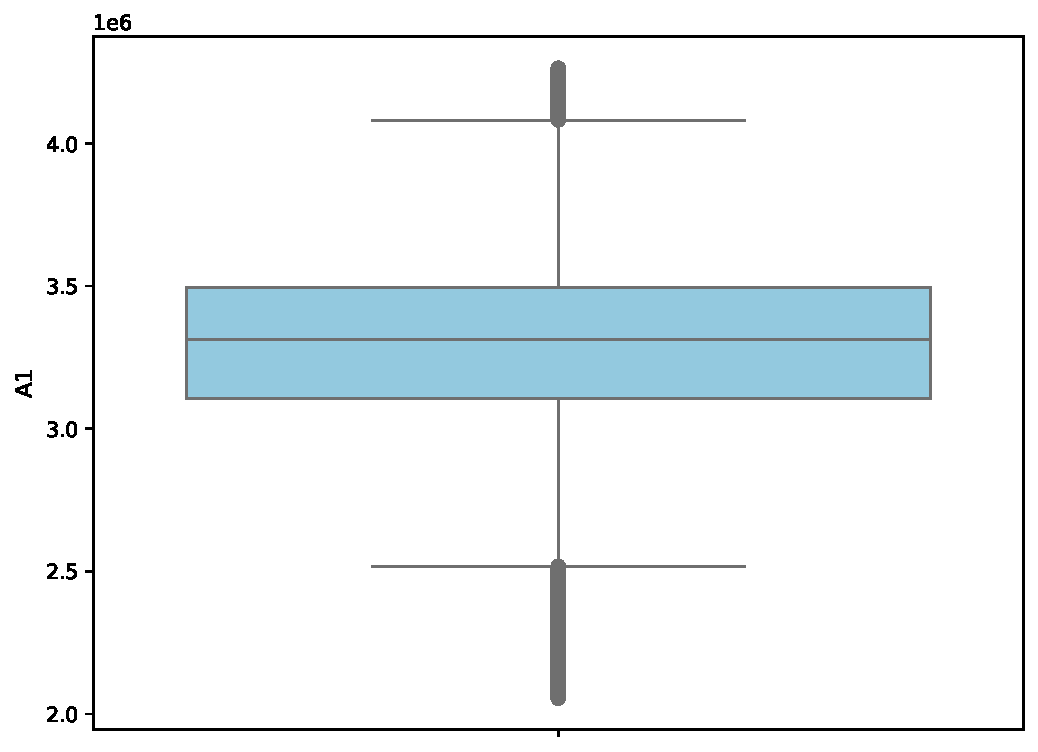
\includegraphics[width=0.6\textwidth]{images/A1_boxplot.pdf}
    \caption{Boxplot of A1.}
    \label{fig:a1_boxplot}
\end{figure}

The boxplot in figure~\ref{fig:a1_boxplot} provides a visual confirmation of the outliers in feature A1. The central box represents the interquartile range (IQR), containing the middle 50\% of the data. The points extending far below and above the whiskers of the box are individual data points identified as outliers. This visualization clearly shows that a significant number of outliers exist at both the lower and upper ends of the distribution.

\begin{figure}[H]
    \centering
    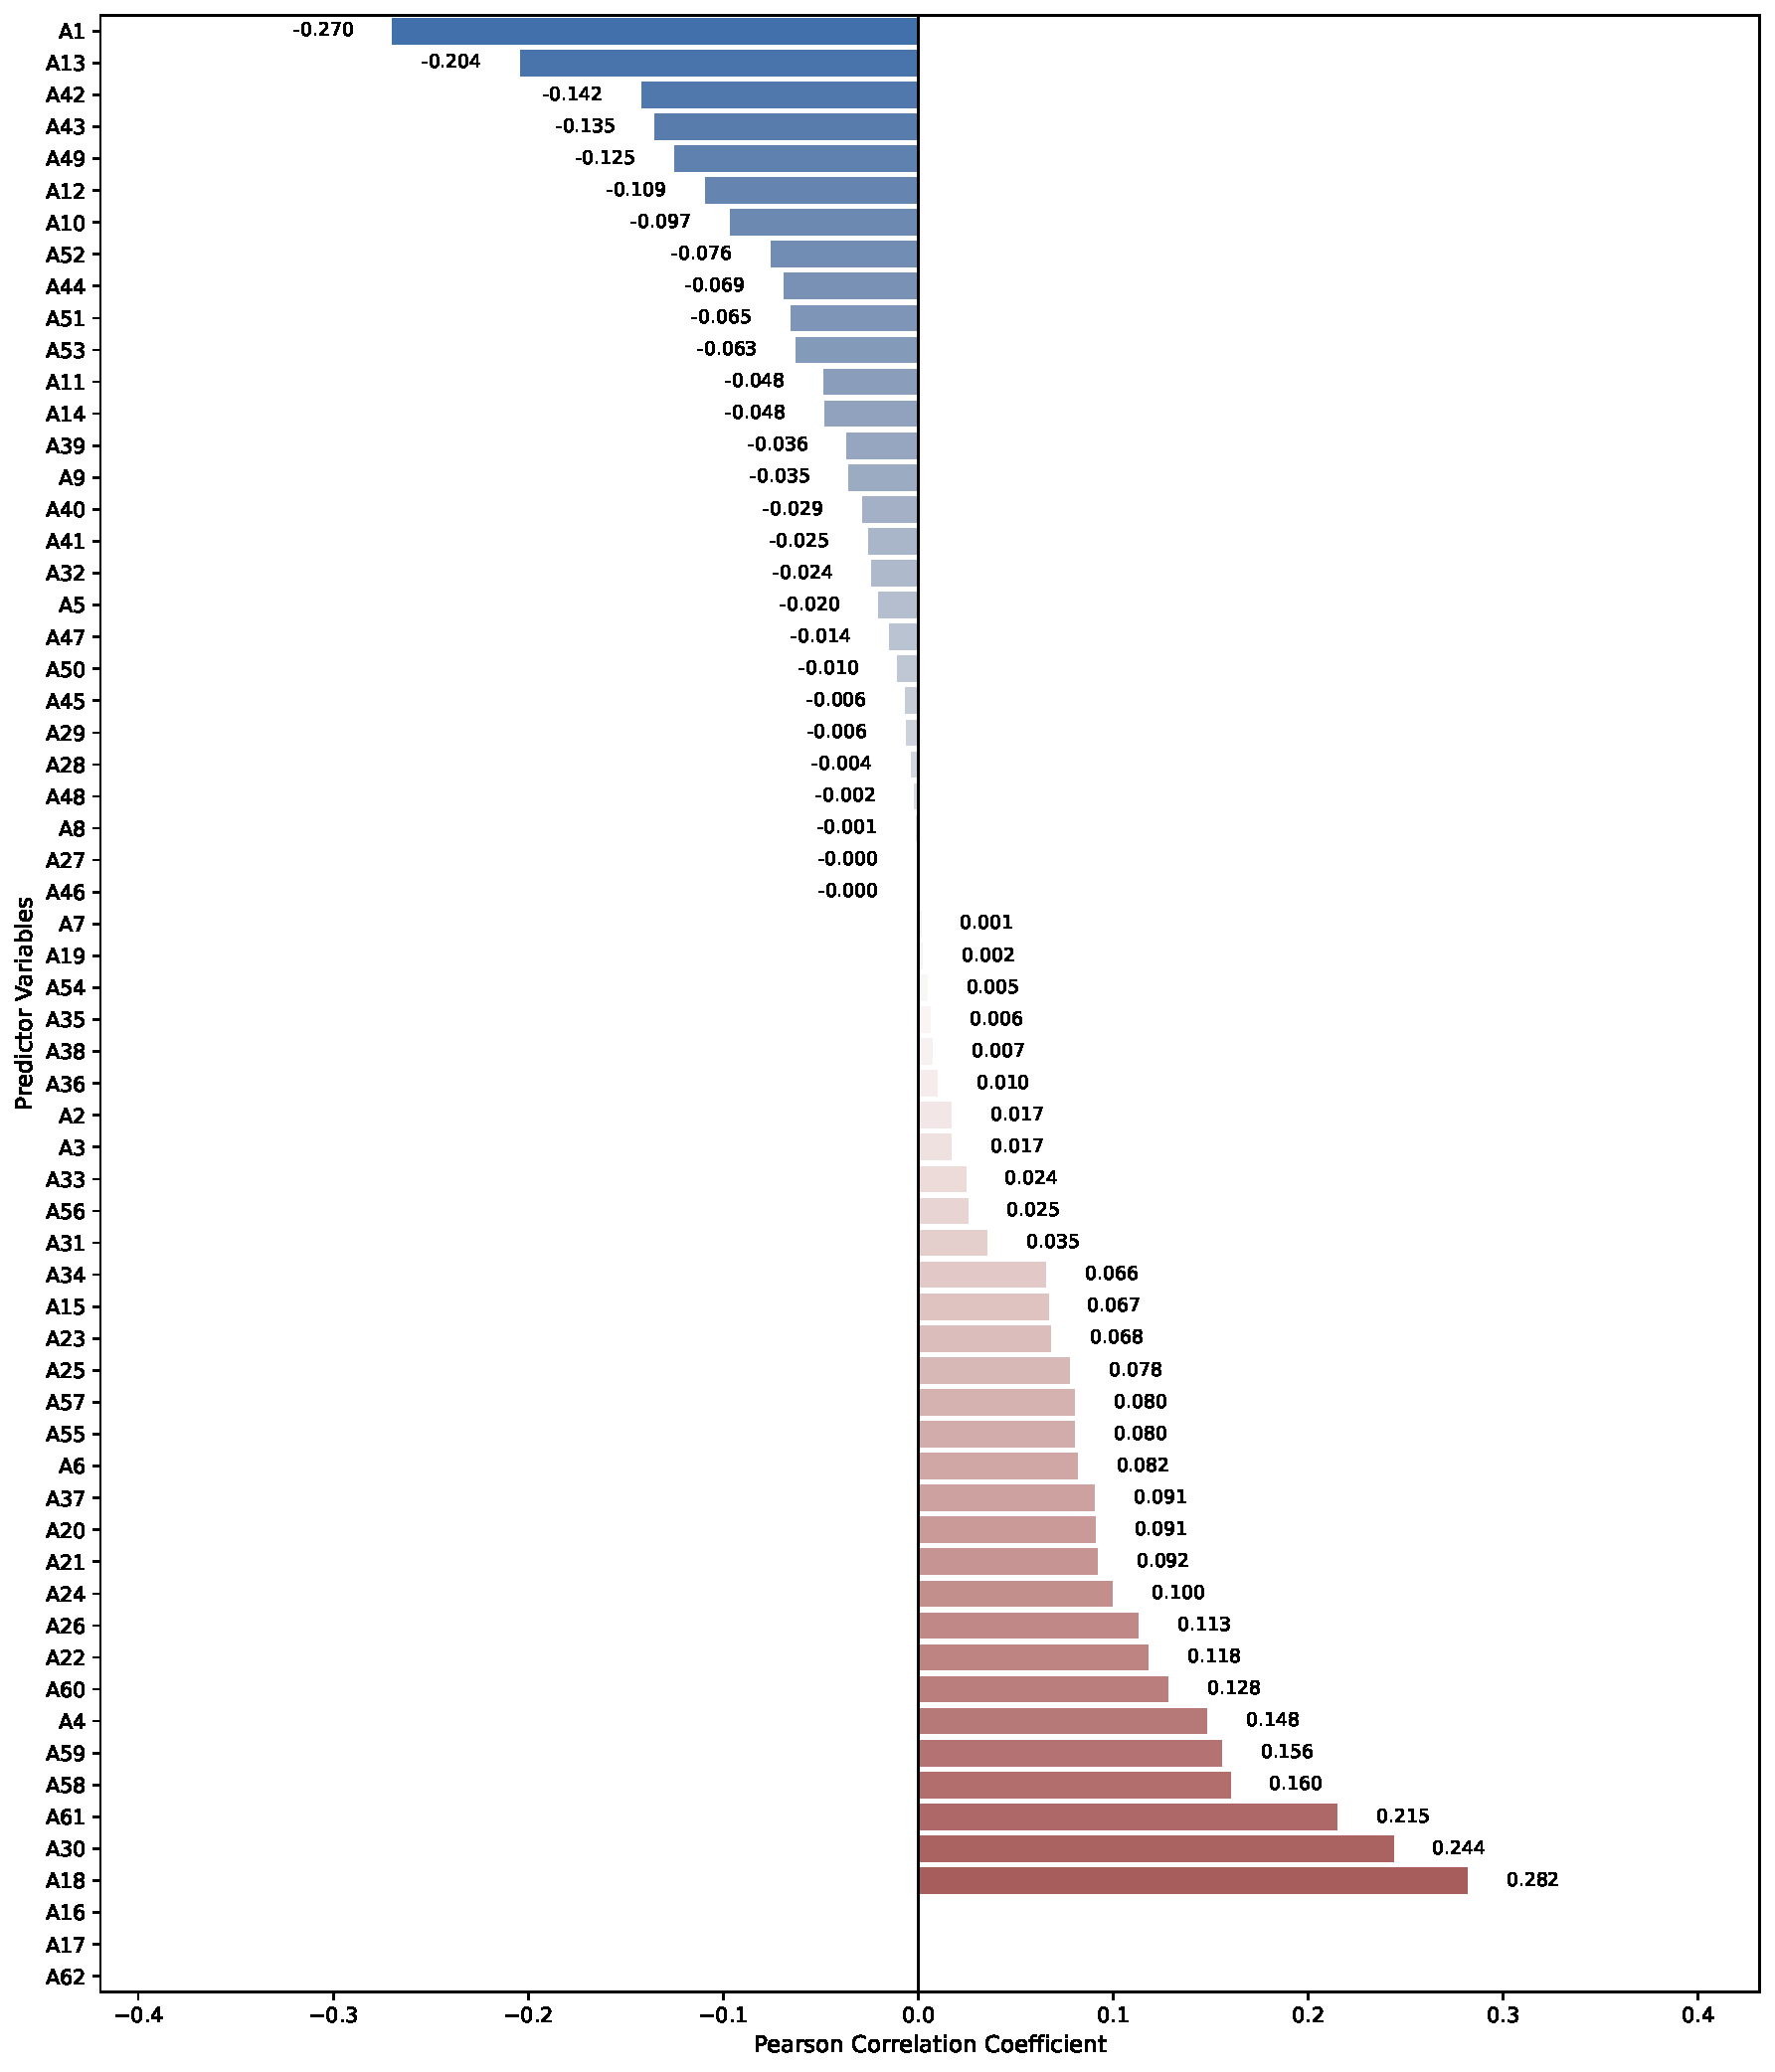
\includegraphics[width=0.6\textwidth]{images/correlation_with_T.pdf}
    \caption{Correlation of Each Predictor with Response Variable.}
    \label{fig:correlation_with_T}
\end{figure}

Figure~\ref{fig:correlation_with_T} illustrates the Pearson correlation coefficient, which measures the linear relationship between each predictor and the response. The analysis shows that most features have a weak to moderate correlation with the response, with all values falling between -0.27 and 0.29. This indicates that no single feature is a dominant predictor, suggesting that an effective model will need to leverage a combination of multiple features.

\begin{figure}[H]
    \centering
    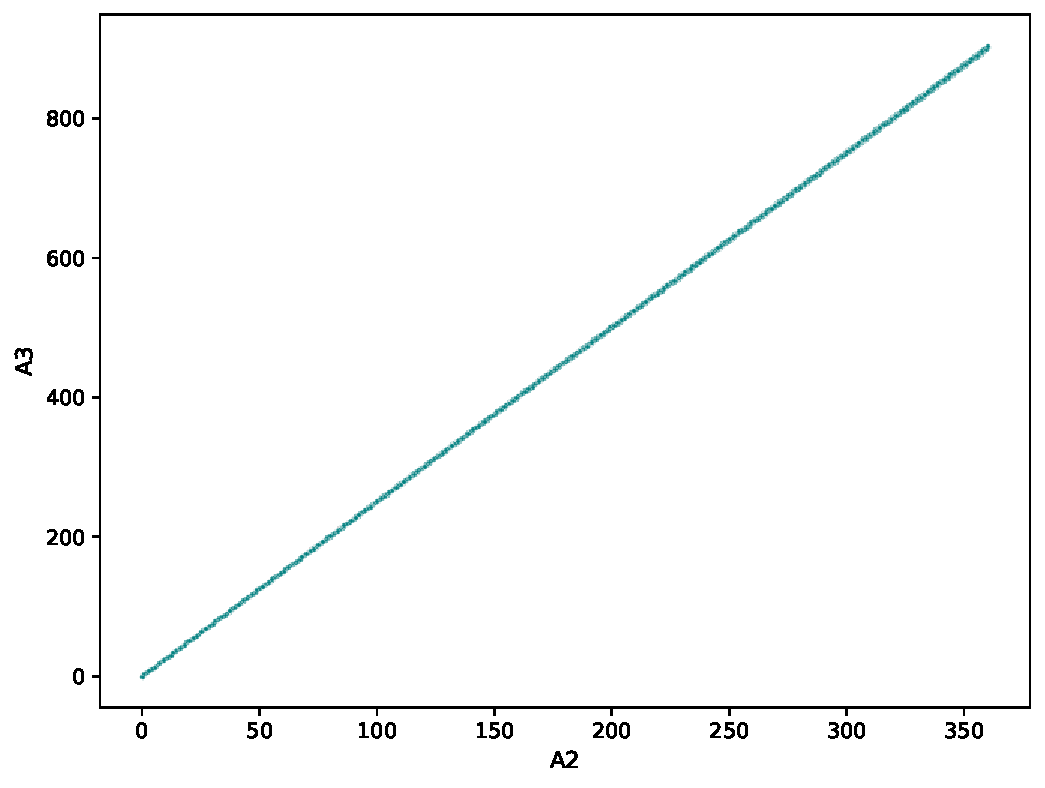
\includegraphics[width=0.6\textwidth]{images/A2_vs_A3_scatterplot.pdf}
    \caption{Scatter plot of A2 vs A3.}
    \label{fig:A2_vs_A3_scatterplot}
\end{figure}

Figure~\ref{fig:A2_vs_A3_scatterplot} shows that there is an extremely strong, positive, and linear relationship between A2 and A3. The line appears to start at the origin which indicates that A3 is just be a scaled version of A2. This means that the two variables are redundant and including both in the dataset does not provide any new information.

\end{document}